\documentclass[12pt,fleqn]{article}
%\usepackage {psfig,epsfig} % para incluir figuras em PostScript
\usepackage{amsfonts,amsthm,amsopn,amssymb,latexsym}
\usepackage{hyperref}
\usepackage{graphicx}
\usepackage[T1]{fontenc}
\usepackage[brazil]{babel}
\usepackage{geometry}
\usepackage{here}
\usepackage[utf8]{inputenc}
\usepackage[intlimits]{amsmath}
\usepackage{subfigure}
%alguns macros
\newcommand{\R}{\ensuremath{\mathbb{R}}}
\newcommand{\Rn}{{\ensuremath{\mathbb{R}}}^{n}}
\newcommand{\Rm}{{\ensuremath{\mathbb{R}}}^{m}}
\newcommand{\Rmn}{{\ensuremath{\mathbb{R}}}^{{m}\times{n}}}
\newcommand{\contcaption}[1]{\vspace*{-0.6\baselineskip}\begin{center}#1\end{center}\vspace*{-0.6\baselineskip}}%================================================================

% Dimensões da página
\usepackage{a4}                       % tamanho da página
\setlength{\textwidth}{16.0cm}        % largura do texto
\setlength{\textheight}{9.0in}        % tamanho do texto (sem head, etc)
\renewcommand{\baselinestretch}{1.15} % espaçamento entre linhas
\addtolength{\topmargin}{-1cm}        % espaço entre o head e a margem
\setlength{\oddsidemargin}{-0.1cm}    % espaço entre o texto e a margem
       
% Ser indulgente no preenchimento das linhas
\sloppy
 

\begin{document}
\pagestyle {empty}

% Páginas iniciais
% capa ilustrativa

\vspace*{-2cm}
{\bf
\begin{center}
{\large
\hspace*{0cm}Instituto Federal de Educação, Ciência e Tecnologia do Ceará} \\
\vspace*{0.3cm}
\hspace*{0cm}Engenharia da computação\\
\hspace*{0cm}  \\
\end{center}}
\vspace{4.0cm}
\noindent
\begin{center}
{\Large \bf Visão Computacional \\ 
\vspace*{1.0cm}
Prof. Pedro Pedrosa \\
\vspace*{1.0cm}
Relatório N$^o$ 2 - Testes com segmentação de imagens} \\[3cm]
{\Large David Paulo Magalhães Araújo}\\[6mm]

\end{center}




{\raggedleft
\begin{minipage}[t]{6.3cm}
\setlength{\baselineskip}{0.25in}

\end{minipage}\\[6cm]}
\vspace{1cm}
{\center Fortaleza \\[3mm]
Abril de 2018 \\}


\newpage
%\pagestyle {empty}
%\abstract{ escrever o resumo do trabalho }

\newpage

\tableofcontents
% Numeração em romanos para páginas iniciais (sumários, listas, etc)
%\pagenumbering {roman}
\pagestyle {plain}

\setcounter{page}{0} \pagenumbering{arabic}

  
\setlength{\parindent}{0in}  %espaco entre paragrafo e margem 
% Espaçamento entre parágrafos
\parskip 5pt  
\newpage
\section{Introdução}

%comando cria itens
% \begin{itemize}
%   \item Filtro da mediana
%   \item apresentar trabalhos relacionados
%   \item apresentar motivação
%   \item apresentar objetivos
%   \item último parágrafo deve conter a organização do documento
%   \item novo item
% \end{itemize}


  \subparagraph{\normalfont Este relatório tem como objetivo principal relatar os resultados dos testes realizados com algoritmos muito utilizados no processo de segmentação de imagens. A seguir, estão listados os algoritmos que serão abordados nesse documento:}

\begin{itemize}
  \item Limiarização local
  \item Crescimento de regiões
  \item Transformada de Hough
\end{itemize}


\section{Testes com Limiarização Local}

  \subparagraph{\normalfont Nessa seção, abordaremos o processo de limiarização local de uma imagem, e compará-la com a limiarização global.}

  \subparagraph{\normalfont Na implementação feita em C, A limiarização local
  pode ser feita carregando uma imagem (opção 0 ou 1), depois selecionando a opção de Limiarização (opção 8). No próximo menu que aparecer, escolher a opção 'local' (opção 1).} 
  

   \subparagraph{\normalfont A limiarização local é uma operação de vizinhança que consiste em determinar se um pixel faz parte de um objeto ou do fundo, dependendo dos valores de sua vizinhança local, em que essa vizinhança pode ser uma janela 3x3, 5x5 etc, o que diferencia-se da limiarização global, em que cada pixel é comparado com um ou mais limiares globais para alcançar o mesmo objetivo. Em ambas os processos, usou-se um limiar de 128 e, na limiarização local, usou-se uma janela 3x3 com um algoritmo simples que tira a média da soma entre o maior e o menor valor de pixel e comparando com o limiar. }
   

  \begin{figure}[!htb]
  \centering
  \subfigure[Imagem original]{
  \hspace{-2cm} 
  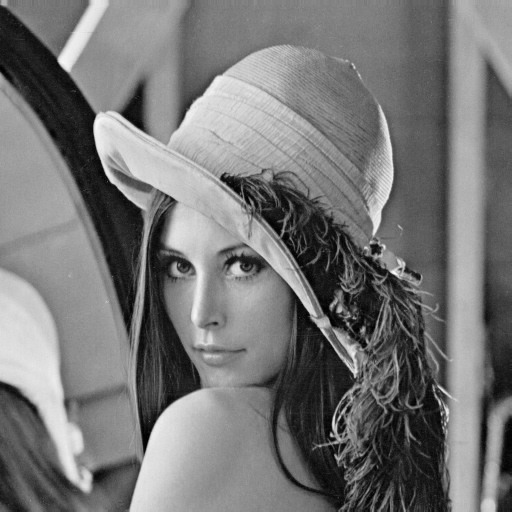
\includegraphics[height=5cm, width=5cm]{images/original.jpg}
  \label{fig:Antes do filtro}
  }\subfigure[Após limiarização global]{
  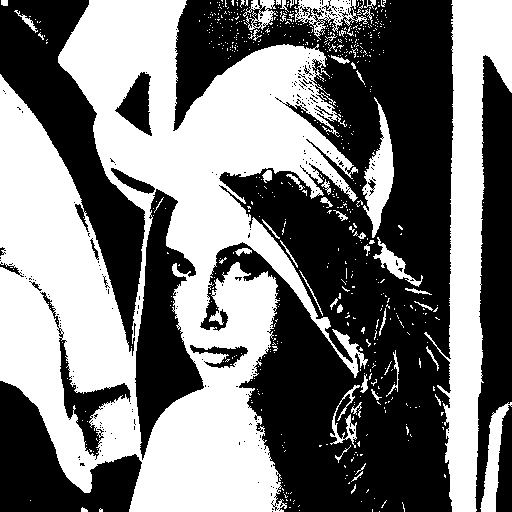
\includegraphics[height=5cm, width=5cm]{images/limiar_global_128.jpg}
  \label{fig:Após limiarização global}  
  }
  \subfigure[Após limiarização local]{
  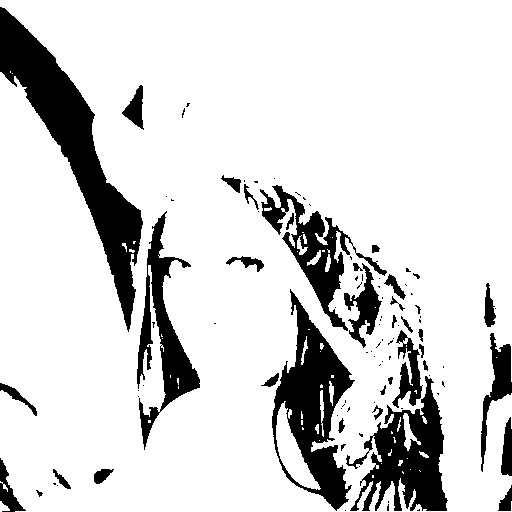
\includegraphics[height=5cm, width=5cm]{images/limiar_3x3_128.jpg}
  \label{fig:Após limiarização local}  
  }
  \caption{Aplicação das limiarizações local e global}
  \label{fig:Resultado 1}
  \end{figure}

  \section{Crescimento de região}

      \subparagraph{\normalfont O algoritmo de crescimento de região consiste em lançar uma semente em uma região da imagem, para que ela cresça por cima de pixels semelhantes ao pixel da semente inicial, até cobrir toda uma região de pixels similares, segmentando uma região da imagem.}
      
      \subparagraph{\normalfont Na aplicação, carregue uma imagem (opção 0 ou 1), selecione a opção 'Crescimento de região' (opção a) e depois informe a localização da semente que irá crescer e delimitar uma região.
      }
     

      \newpage

      \begin{figure}[!htb]
      \centering
      \subfigure[Imagem original]{
      \hspace{-2cm} 
      
\includegraphics[height=5cm, width=5cm]{images/shapes.png}
      \label{fig:Antes do filtro}
      }\subfigure[Região segmentada em preto]{
      
\includegraphics[height=5cm, width=5cm]{images/reggrowth.jpg}
      \label{fig:Depois do filtro}  
      }
      \caption{Resultado do crescimento da semente dentro do círculo}
      \label{fig:Resultado 1}
      \end{figure}
      

  \section{Transformada de Hough}

      \subparagraph{\normalfont A transformada de Hough é uma técnica de extração de atributos usada em processamento de imagens. O propósito da técnica é encontrar instâncias de objetos dentro de uma certa classe de formatos através de um mecanismo de 'voto'. Atraves desse mecanismo, é gerado um vetor acumulador, em que é possível detectar possíveis instâncias do objeto na imagem.}
      
      \subparagraph{\normalfont Na aplicação, é possível verificar o exemplo abaixo carregando a imagem shapes.png (opção 1), e selecionando a opção 'Transformada de Hough' (opção b)}

      \newpage

      \begin{figure}[!htb]
      \centering
      \subfigure[Imagem]{
      \hspace{-2cm} 
      
\includegraphics[height=5cm, width=5cm]{images/lines.png}
      \label{fig:Antes do filtro}
      }\subfigure[Vetor Acumulador]{
      
\includegraphics[height=5cm, width=5cm]{images/hough_transf.jpg}
      \label{fig:Depois do filtro}  
      }
      \caption{Resultado da transformada de Hough}
      \label{fig:Resultado 1}
      \end{figure}


\section{Resumo Geral}

  \subparagraph{\normalfont Esse documento faz um breve relatório dos resultados obtidos pela implementação em C dos processos de segmentação de imagem abordados por ele. 
  No decorrer do relatório, é possível notar que os resultados obtidos estão dentro do esperado para os testes realizados, vinculando teoria e prática como eram os objetivos do documento.}

  \subparagraph{\normalfont O documento ensina, também, como usar a implementação feita em C para verificar os testes que foram feitos e comparar com os resultados obtidos.}

\section{Referências}

Transformada de Hough (em inglês): \\
\href{https://homepages.inf.ed.ac.uk/rbf/HIPR2/hough.htm}
{\textit{https://homepages.inf.ed.ac.uk/rbf/HIPR2/hough.htm}} \\

Aula 8 da cadeira de visão computacional do IFCE: \\
\href{https://www.dropbox.com/s/xiyfnwxb2z5cez4/VC\%20-\%20Aula\%208\%20-\%20Segmentacao.pdf?dl=0}{\textit{https://www.dropbox.com/s/xiyfnwxb2z5cez4/VC\%20-\%20Aula\%208\%20-\%20Segmentacao.pdf?dl=0}} \\



\bibliographystyle{unsrt}
\bibliography{bibliografia}





% %\label{sec:tab}
% \begin{table}[htb]
% \caption{Tabela de Exemplo...}
% \label{tab:Ex1}
% \begin{center}
% 		\begin{tabular}{@{}lcccccc@{}}\hline
% 		  & IRIS (binário) & IRIS & Coluna & Dermatologia &  OR \\\hline \hline
% 		Número de Padrões   & 150 & 150 & 310 & 358 & 80 \\\hline
% 		Número de Atributos & 4   & 4   & 6   & 34  & 2 \\\hline
% 		Número de Classes   & 2   & 3   & 3   & 6   & 2 \\\hline
% 		\end{tabular}
% \end{center}
% \end{table}


% \begin{equation}
%   \label{eq:ex1}
%   A=B+C
% \end{equation}

% \begin{equation}
%   \label{eq:ex2}
%   \sigma = \mu + \delta
% \end{equation}

% Para citar trechos das fórmulas no texto basta colocar o que quer citar entre cifrão ``\$'' (ver o código do latex para citar o $\sigma$, $\mu$ e $\delta$ sem estar dentro de equações). 

% Para citar equações, tabelas e figuras, deve-se usar $\ $$\ $ref e colocar a label que identifica cada um destes elementos. Por exemplo, Figura \ref{fig:FigExMulti1}, Tabela \ref{tab:Ex1}, Equações \ref{eq:ex1} e \ref{eq:ex2}. 

% \begin{figure}[!htb]
% \centering
% \subfigure[Íris 2-Classes]{
% \hspace{-2cm} 
% \includegraphics[scale=0.3]{fig/fig1a.png}
% \label{fig:FigExMulti1a}
% }\subfigure[Íris 3-Classes]{
% \includegraphics[scale=0.3]{fig/fig1b.png}
% \label{fig:FigExMulti1b}  
% }
% \caption{Exemplo de multiplas figuras 1.}
% \label{fig:FigExMulti1}
% \end{figure}

% \begin{figure}[!htb]
%    \centering
%    \subfigure[]{\label{fig:FigExMulti2a}\includegraphics[width=0.4\hsize]{fig/fig1a.png}}
%    \hspace{0.005\hsize}
%    \subfigure[]{\label{fig:FigExMulti2b}\includegraphics[width=0.4\hsize]{fig/fig1b.png}}
%    \caption{Exemplo 2 de figuras multiplas.}
%    \label{ex3dDetails}
% \end{figure}

% \begin{figure}[!hbt]
% \begin{center}
% \includegraphics[scale=0.2]{fig/fig1a.png}
% \end{center}
% \caption{\label{ExfigIndividual}\hspace{-0.4em} Exemplo de como adicionar figuras individuais.}
% \end{figure}

% %\clearpage

% \section{Sites que ajudam na escrita com Latex} 

% Nas subseções à seguir estão sites para ajudar a fazer equações e tabelas.

% \subsection{Sites para fazer Equações}

% Site 1:

% \href{http://www.codecogs.com/latex/eqneditor.php?lang=pt-br}{\textit{http://www.codecogs.com/latex/eqneditor.php?lang=pt-br}}

% Site 2:

% \href{http://www.hostmath.com}{\textit{http://www.hostmath.com}}

% \subsection{Sites para fazer Tabelas}

% Site 1:

% \href{http://www.tablesgenerator.com}{\textit{http://www.tablesgenerator.com}}

% Site 2: 

% \href{http://truben.no/table/}{\textit{http://truben.no/table/}}

% Site 3:

% \href{http://truben.no/table/old/}{\textit{http://truben.no/table/old/}}

% \section{Editores de Latex}

% O mais usado editor de latex on line e gratuito é o Overleaf (\href{https://www.overleaf.com}{\textit{https://www.overleaf.com}}). Basta criar um novo projeto e fazer upload da pasta do projeto zipado, que o projeto é carregado e habilitado para edição online na plataforma. Existe outros Editores de texto em latex, mas o overleaf facilita o uso por ser gratuito e on line.

% \section{Referências Bibliográficas}

%  As referências são necessárias para embasar o conteúdo que está sendo discutido, principalmente detalhes técnicos que estão em destaque. As referências são inseridas usando o comando $\ $cite, e já gera a lista de referências no fim seguindo o modelo (template) usado. Abaixo seguem alguns exemplos (veja o código do arquivo *tex).
 
%  Quando eu quero resumir ou destacar algo de algum artigo, livro eu adiciono tal citação, como por exemplo \cite{Adler89} (veja o código do arquivo *tex).
 

% \section{Resumo Geral}

% Após apresentar os cálculos para cada simulação, apresente as respectivas simulações, inclusive com todas as variações possíveis, discutindo e/ou apresentando alguma conclusão sobre as simulações relacionando com a teoria. 

% \bibliographystyle{unsrt}
% \bibliography{bibliografia}

\end{document} %finaliza o documento
